\section{Analisi}

\subsection{Script e Configurazione dei Test}

Per gestire l'esecuzione di un vasto numero di test con configurazioni eterogenee, è stato implementato un processo automatizzato orchestrato dallo script \texttt{scripts/run.sh}. La sua esecuzione può essere suddivisa nelle seguenti fasi:

\begin{enumerate}
    \item \textbf{Inizializzazione e Pulizia:} La prima azione dello script è la preparazione dell'ambiente di esecuzione. Vengono rimossi i risultati di esecuzioni precedenti eliminando il contenuto delle directory \texttt{logs/ csv/ plots/ profiling/ bin/}, se in caso queste non dovessero esistere verranno create. Questo garantisce che ogni esecuzione parta da uno stato pulito e che i risultati non vengano contaminati da test precedenti.

    \item \textbf{Compilazione:} Viene compilato il codice sorgente presente nella directory \texttt{src/} usando \texttt{nvcc}. L'eseguibile risultante, \texttt{bin/main.out}, viene così aggiornato all'ultima versione del codice prima dell'avvio dei test.

    \item \textbf{Iterazione sui File di Configurazione:} Lo script itera su tutti i file con estensione \texttt{.csv} presenti nella directory \texttt{tests/}. Ciascun file definisce una famiglia di test; al suo interno, ogni riga (esclusa l'intestazione) specifica i parametri per una singola esecuzione.

    \item \textbf{Generazione e Sottomissione dei Job:} Per ogni riga di un file di configurazione, che rappresenta un singolo test, lo script esegue i seguenti passaggi:
          \begin{itemize}
              \item \textbf{Parsing dei Parametri:} I valori per \texttt{matrix\_size}, \texttt{n\_proc}, \texttt{n\_gpu}, \texttt{tile\_width}, \texttt{grid\_width} e \texttt{grid\_height} vengono estratti dalla riga corrente.
              \item \textbf{Creazione dello Script SLURM:} Viene generato dinamicamente uno script di sottomissione SLURM. Questo script contiene le direttive \texttt{\#SBATCH} necessarie per richiedere le risorse al cluster (nodi, task, GPU per task) e definire i file di output e di errore. Il comando di esecuzione principale è incapsulato da \texttt{nsys profile} per la profilazione, e l'eseguibile \texttt{bin/main.out} viene lanciato con i parametri specifici del test.
              \item \textbf{Sottomissione del Job:} Lo script SLURM appena creato viene sottomesso al gestore di code tramite il comando \texttt{sbatch}. L'ID del job restituito da SLURM viene catturato e memorizzato.
              \item \textbf{Gestione delle Dipendenze:} L'ID del job viene aggiunto a una lista di dipendenze che sarà utilizzata nella fase finale.
          \end{itemize}

    \item \textbf{Job di Analisi e Plotting:} Una volta che tutti i job di calcolo sono stati sottomessi, lo script genera un ultimo job SLURM. Questo job ha una dipendenza di tipo \texttt{afterok} da tutti i job sottomessi in precedenza. Ciò significa che verrà eseguito solo dopo che tutti i test di calcolo saranno terminati con successo. Il compito di questo job finale è eseguire lo script Python \texttt{scripts/plots.py}, che si occupa di aggregare i dati dai file \texttt{.csv} generati e di creare i grafici di performance.
\end{enumerate}

\subsection{Analisi delle misurazioni}
Purtroppo, a causa di problemi tecnici con la versione di OpenMPI presente sul cluster, non è stato possibile valutare in maniera significativa il programma. In particolare, la funzione usata per creare la griglia di processi\footnote{\url{https://docs.open-mpi.org/en/v5.0.x/man-openmpi/man3/MPI_Cart_create.3.html}} potrebbe fallire arbitrariamente causando la chiusura forzata dell'eseguibile. Sperimentazioni ausiliarie hanno portato eventualmente sempre allo stesso errore, il che fa presagire qualche problema in quella versione della libreria.

È stato deciso di eseguire dei test locali su una singola macchina, che ovviamente non saranno indicativi delle prestazioni reali ma utili comunque a ricavare qualche spunto di riflessione.
Sono stati eseguiti i seguenti test:
\begin{enumerate}
    \item al crescere del numero di processi e threads, con dimensione fissata
          \begin{enumerate}
              \item al crescere del numero di processi, con numero di thread per processi fissato e
                    dimensione fissata;
              \item al crescere del numero di thread per processo, con numero di processi fissato e
                    dimensione fissata;
          \end{enumerate}
    \item fissata la dimensione del problema per processo, al crescere del numero di processi, con numero di thread per processo fissato;
    \item fissata la dimensione del problema per thread, al crescere del numero di thread, con numero di processi fissato;
    \item fissata la dimensione del problema per thread, al crescere del numero di processi, con numero di thread per processo fissato.
\end{enumerate}

% \begin{table}[h]
%     \centering
%     \begin{tabular}{|l|l|}
%         \hline
%         Matrice            & Tempo (s)  \\ \hline
%         $64   \times 64  $ & 0.000572   \\ \hline
%         $128  \times 128 $ & 0.004717   \\ \hline
%         $256  \times 256 $ & 0.035934   \\ \hline
%         $512  \times 512 $ & 0.285774   \\ \hline
%         $1024 \times 1024$ & 2.272720   \\ \hline
%         $1448 \times 1448$ & 6.429910   \\ \hline
%         $2048 \times 2048$ & 18.552951  \\ \hline
%         $2896 \times 2896$ & 52.893937  \\ \hline
%         $4096 \times 4096$ & 152.709002 \\ \hline
%     \end{tabular}
%     \caption{Prestazioni algoritmo sequenziale}
% \end{table}

% \begin{table}[h]
%     \begin{tabular}{|c|c|c|c|c|c|c|}
%         \hline
%         Matrice    & Processi & Blocchi & Thread & GPU (s)  & Kernel (s) & cuBLAS (s) \\ \hline
%         $ 2048^2 $ & 2        & 1       & 1024   & 2.317158 & 2.200990   & 0.286483   \\ \hline
%         $ 2048^2 $ & 4        & 1       & 1024   & 2.234591 & 2.078579   & 0.274687   \\ \hline
%         $ 2048^2 $ & 8        & 1       & 1024   & 2.278694 & 2.010755   & 0.325228   \\ \hline
%         $ 2048^2 $ & 16       & 1       & 1024   & 2.438489 & 1.928693   & 0.351413   \\ \hline
%     \end{tabular}
%     \caption{1a}
% \end{table}

% \begin{table}[h]
%     \begin{tabular}{|c|c|c|c|c|c|}
%         \hline
%         Matrice    & Processi & Blocchi & Thread & GPU (Kernel)            & cuBLAS     \\ \hline
%         $ 2048^2 $ & 4        & 1       & 1024   & 2.317158 s (2.200990 s) & 0.286483 s \\ \hline
%         $ 2048^2 $ & 4        & 4       & 1024   & 2.234591 s (2.078579 s) & 0.274687 s \\ \hline
%         $ 2048^2 $ & 4        & 8       & 1024   & 2.278694 s (2.010755 s) & 0.325228 s \\ \hline
%         $ 2048^2 $ & 4        & 16      & 1024   & 2.438489 s (1.928693 s) & 0.351413 s \\ \hline
%     \end{tabular}
%     \caption{1b}
% \end{table}

\begin{figure}[h]
    \centering
    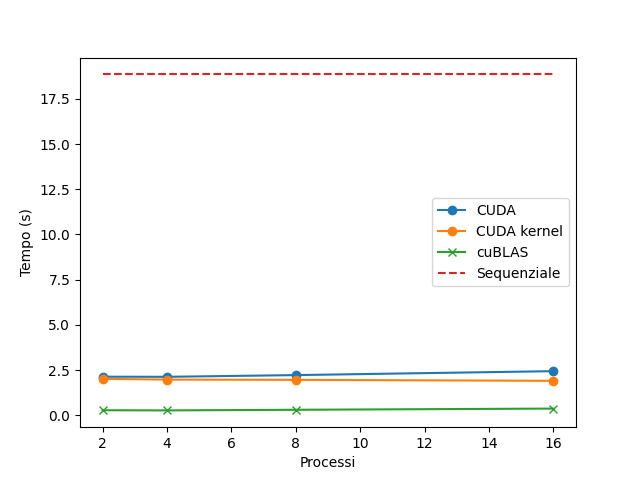
\includegraphics[width=0.7\textwidth]{./imgs/graphs/caso_a1.png}
    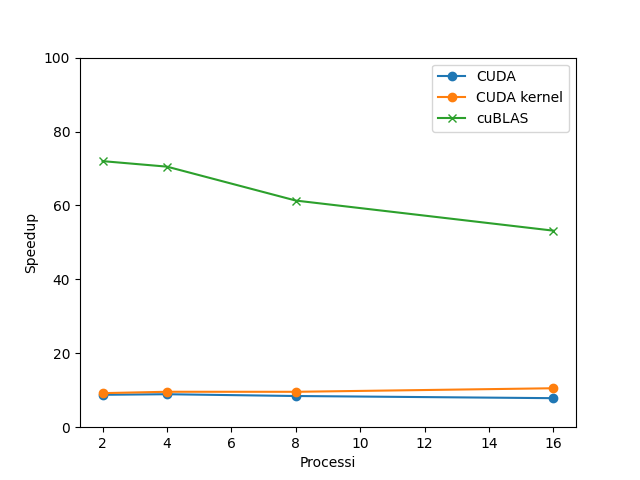
\includegraphics[width=0.7\textwidth]{./imgs/graphs/caso_a1_speedup.png}
    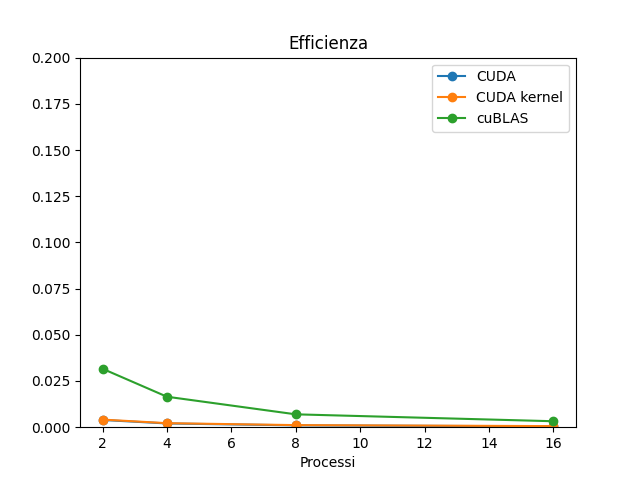
\includegraphics[width=0.7\textwidth]{./imgs/graphs/caso_a1_efficiency.png}
    \caption{Caso 1a}
\end{figure}

\begin{figure}[h]
    \centering
    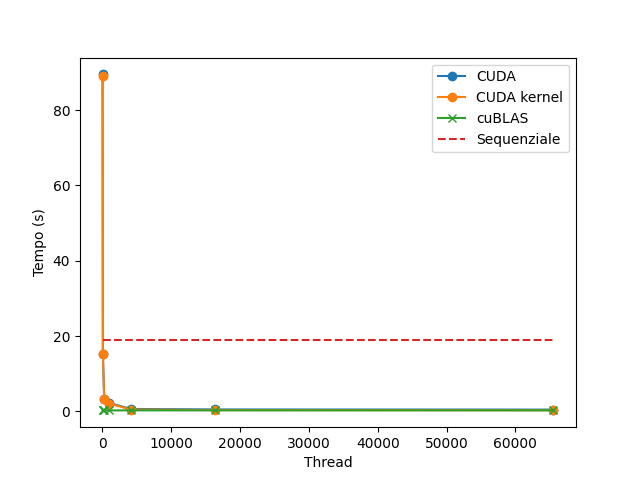
\includegraphics[width=0.7\textwidth]{./imgs/graphs/caso_a2.png}
    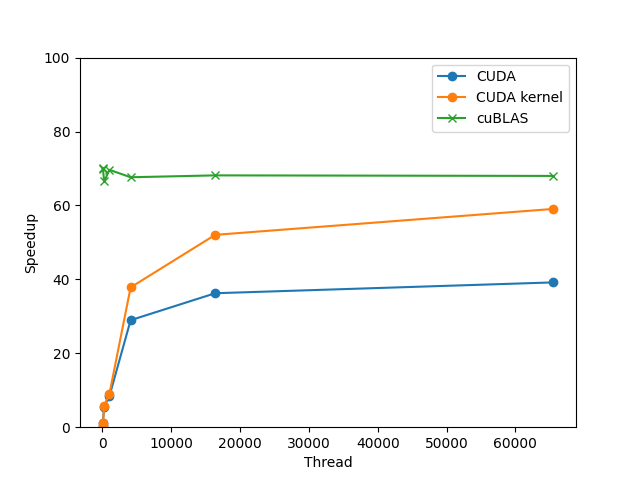
\includegraphics[width=0.7\textwidth]{./imgs/graphs/caso_a2_speedup.png}
    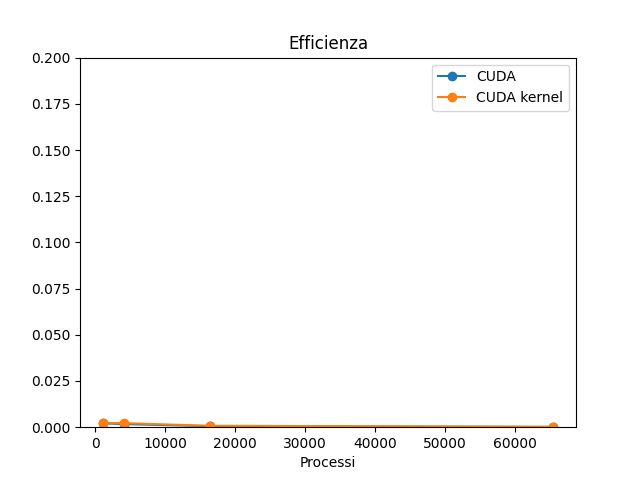
\includegraphics[width=0.7\textwidth]{./imgs/graphs/caso_a2_efficiency.png}
    \caption{Caso 1b}
\end{figure}

\begin{figure}[h]
    \centering
    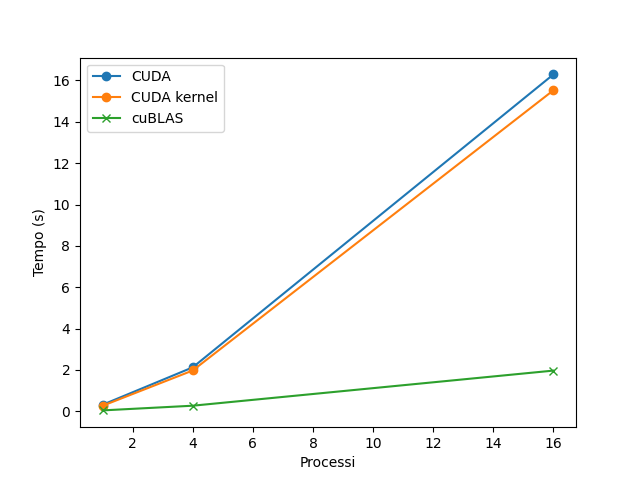
\includegraphics[width=0.7\textwidth]{./imgs/graphs/caso_b.png}
    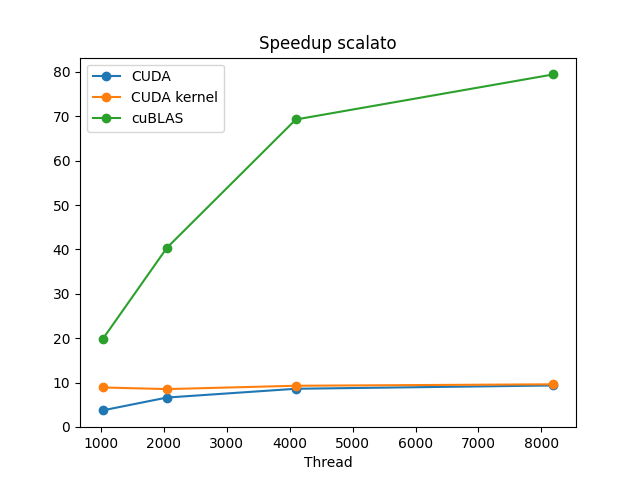
\includegraphics[width=0.7\textwidth]{./imgs/graphs/caso_b_scaled_speedup.png}
    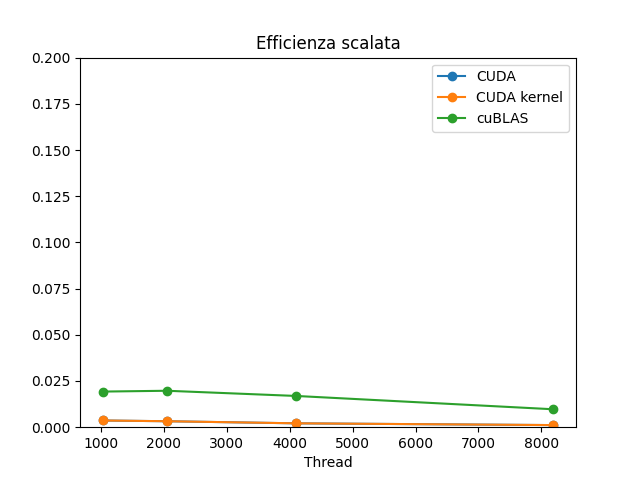
\includegraphics[width=0.7\textwidth]{./imgs/graphs/caso_b_scaled_efficiency.png}
    \caption{Caso 2}
\end{figure}

\begin{figure}[h]
    \centering
    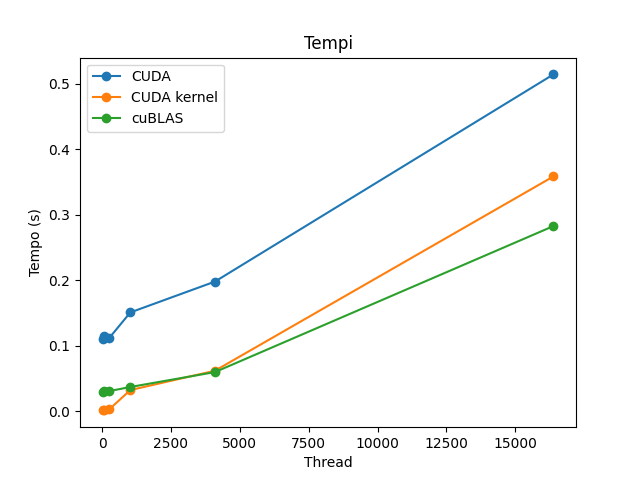
\includegraphics[width=0.7\textwidth]{./imgs/graphs/caso_c.png}
    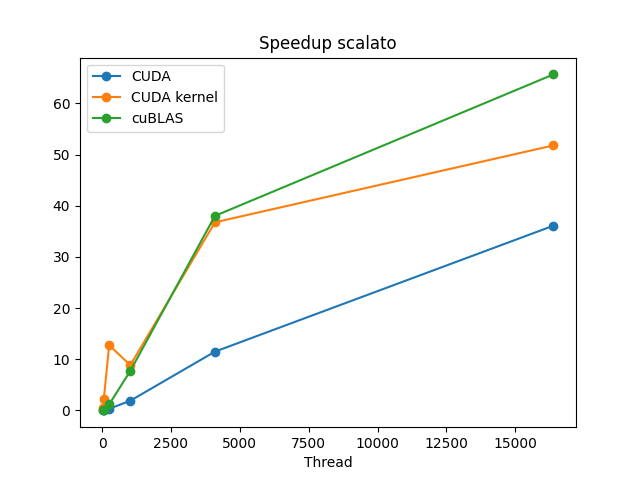
\includegraphics[width=0.7\textwidth]{./imgs/graphs/caso_c_scaled_speedup.png}
    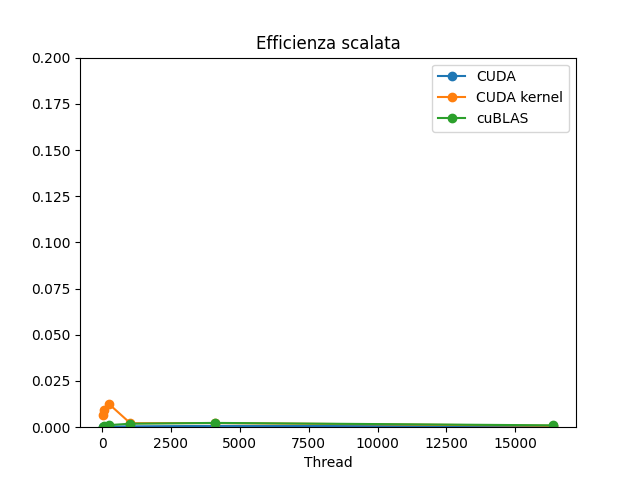
\includegraphics[width=0.7\textwidth]{./imgs/graphs/caso_c_scaled_efficiency.png}
    \caption{Caso 3}
\end{figure}

\begin{figure}[h]
    \centering
    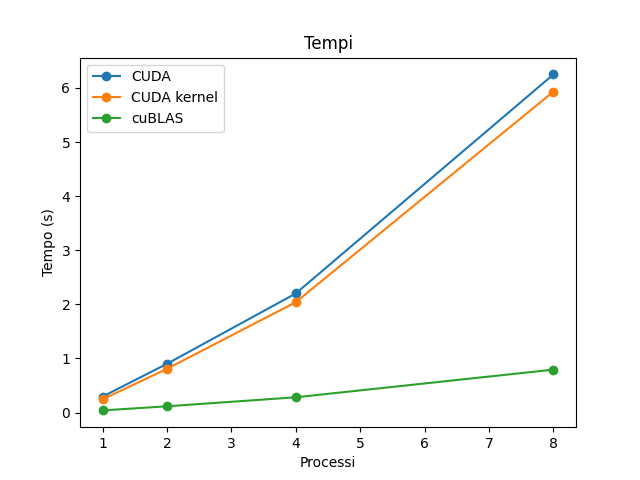
\includegraphics[width=0.7\textwidth]{./imgs/graphs/caso_d.png}
    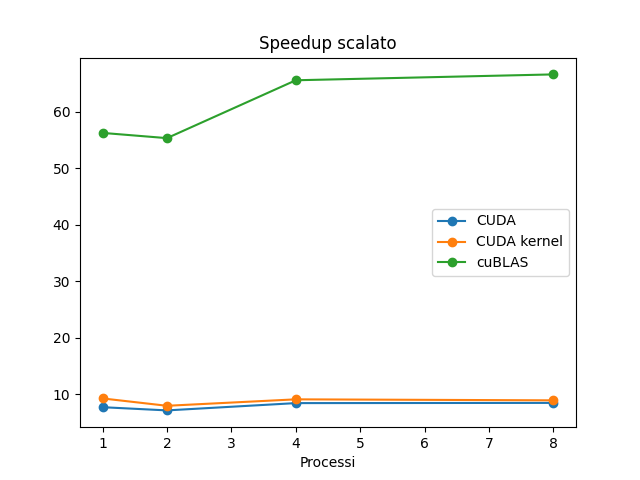
\includegraphics[width=0.7\textwidth]{./imgs/graphs/caso_d_scaled_speedup.png}
    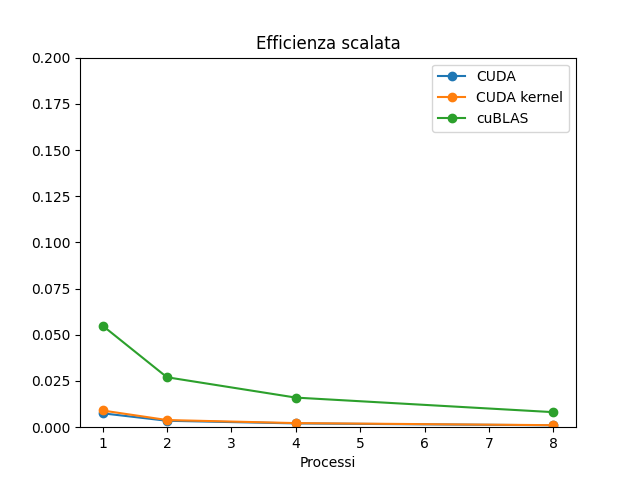
\includegraphics[width=0.7\textwidth]{./imgs/graphs/caso_d_scaled_efficiency.png}
    \caption{Caso 4}
\end{figure}

Non è possibile trarre conclusioni certe date le limitazioni del caso ma un risultato ovvio è il miglioramento dei tempi di esecuzione grazie al parallelismo offerto dalle GPU.
In caso di un singolo nodo a parità di dimensioni della matrice, conviene aumentare il numero di thread usati dalla GPU piuttosto che distribuire il carico aumentando i processi. Ciò probabilmente è dovuto al fatto che i processi non riescono a utilizzare tutti contemporaneamente la GPU causando delle attese.

Un risultato leggermente preoccupante è l'efficienza praticamente nulla ottenuta dai vari test.

L'implementazione cuBLAS risulta, come prevedibile, molto ottimizzata e migliore della semplice implementazione presa in questione.

\subsection{NVIDIA Nsight Compute}

NVIDIA Nsight Compute è un profiler per CUDA che fornisce metriche dettagliate delle prestazioni e debug delle API tramite interfaccia utente e strumenti da riga di comando.
% TODO: che altro?

Purtroppo, a causa dei problemi tecnici riportati precedentemente, non è stato possibile valutare le metriche fornite da queste applicazioni.
